\documentclass[aspectratio=169,xcolor=dvipsnames]{beamer}
% https://github.com/PM25/SimplePlus-BeamerTheme
\usetheme{SimplePlus}

\usepackage{hyperref}
\usepackage{graphicx} 
\usepackage{booktabs}
\usepackage{courier}

\usepackage[spanish]{babel}

% Portada

\title{\large Diseño y desarrollo de un microservicio para la gestión de información de monitorización y predicciones de tráfico en red}

\author{\small \textit{Autor}: Enrique Fernández Sánchez \\
\textit{Tutor}: Pablo Pavón Mariño}

\institute[UPCT]{\\ Universidad Politécnica de Cartagena (UPCT) \\ \vspace{5px}
	
\includegraphics[scale=0.2]{img/escudo_upct.png}
}

\date{\today}

\usepackage{tikz}
\logo{ 
	\begin{tikzpicture}[overlay,remember picture, inner sep=0pt,outer sep=0pt]
		\node[yshift=-20px,left=0.2cm] at (current page.31){
			
\includegraphics[width=3cm]{img/etsit.png}
		};
	\end{tikzpicture}
}

\begin{document}
	% 1
	\begin{frame}
		\titlepage
	\end{frame}

	% 2
	\begin{frame}{Índice}
		\tableofcontents
	\end{frame}

    % --------------------
    \section{Introducción}
    
    \begin{frame}{Introducción}
    
        \begin{itemize}
            \item \textit{Abstract}: Aplicación que permite almacenar muestras de monitorización de tráfico en red, y a su vez, generar predicciones futuras del tráfico de red, en función de la información almacenada.
        \end{itemize}
    
        \begin{block}{Objetivos del proyecto}
            \begin{itemize}
                \item Diseñar una \textbf{aplicación} siguiendo la metodología de \textbf{microservicios}.
                
                \item Investigar herramientas de \textbf{predicción de series temporales}.
                
                \item Investigar \textbf{opciones de almacenamiento} para \textbf{muestras temporales}.
                
                \item Utilizar \textbf{herramientas de documentación} que permitan conocer la estructura de la aplicación.\\
                
            \end{itemize}
        \end{block}
    \end{frame}

	% ---------------------
	
	\section{Tecnologías empleadas}

	\begin{frame}{Microservicios}
		\begin{exampleblock}{Definición de microservicio}
			Sistemas que cumplen las siguientes premisas: 
			
			\begin{itemize}
				\item Sistemas pequeños, independientes y poco ``acoplados''. 
				\item Código fuente separado entre los diferentes servicios, no necesariamente mismo lenguaje.
				\item Los servicios se comunican entre sí utilizando APIs.
				\item Cada sistema es independiente, y responsable de su persistencia de datos.
			\end{itemize}
		\end{exampleblock}
		
		\begin{alertblock}{Importancia microservicios}
			content...
		\end{alertblock}
	\end{frame}

	% ---------------------
	
	\begin{frame}{\texttt{API} \small (\textit{Application Programing Interface})}
		\begin{itemize}
			\item Una API permite a dos \textbf{componentes comunicarse} entre sí \textbf{mediante} una serie de \textbf{reglas}.
			
			\item Supone un ``\textbf{contrato}'' en el que \textbf{se establecen las solicitudes} y respuestas \textbf{esperadas en la comunicación}.
		\end{itemize}
	
		\begin{exampleblock}{Tipos de API}
			Dependiendo de la implementación, distinguimos entre cuatro tipos:
			
			\begin{itemize}
				\item \textbf{SOAP}.
				\item \textbf{RPC}.
				\item \textbf{Web Socket}.
				\item \textbf{REST}.
			\end{itemize}
		\end{exampleblock}
	\end{frame}
	
	% ---------------------
	
	\begin{frame}{Bases de datos}
		
		\begin{itemize}
			\item En función del tipo de dato a almacenar, se distinguen dos bases de datos dentro de la aplicación:
		\end{itemize}
		
		\begin{columns}
			\begin{column}{0.5\textwidth}
				\begin{block}{Tipo relacional}
					asdasdasda
				\end{block}
			\end{column}
			
			
			\begin{column}{0.5\textwidth}
				\begin{block}{Tipo serie temporal}
					content...
				\end{block}
			\end{column}
		\end{columns}
	\end{frame}
	
	% ---------------------
	
	\begin{frame}{Lenguaje de programación \& frameworks}
		\begin{columns}
			\begin{column}{0.5\textwidth}
				\begin{exampleblock}{\texttt{Python}}
					Lenguaje de programación orientado a objetos, interpretado y de alto nivel. Muy popular en los siguientes ambitos:
					
					\begin{itemize}
						\item Aplicaciones web.
						
						\item Data Science
						
						\item Inteligencia Artificial
					\end{itemize}
					
					\begin{figure}[h!]
						\begin{center}
							
\includegraphics[width=0.7\textwidth]{img/python_logo.png}
							%\caption{asd}
							%\label{img: microservice architecture}
						\end{center}
					\end{figure}
				\end{exampleblock}
			\end{column}
		
			\begin{column}{0.5\textwidth}
				\begin{exampleblock}{\texttt{FastAPI}}
					Framework moderno y rápido para construir APIs. Características:
					
					\begin{itemize}
						\item Rápido: rendimiento equivalente a otros lenguajes (NodeJS o Go).
						\item Intuitivo: soporta autocompletado. 
						\item Robusto: herramienta Swagger/ReDoc automática.
					\end{itemize}
					
					\begin{figure}[h!]
						\begin{center}
							
\includegraphics[width=0.8\textwidth]{img/fastapi_logo.png}
							%\caption{asd}
							%\label{img: microservice architecture}
						\end{center}
					\end{figure}
				\end{exampleblock}
				
				
			\end{column}
		\end{columns}
	\end{frame}

	\begin{frame}{Lenguaje de programación \& frameworks}
		\begin{exampleblock}{\texttt{Prophet}}
			Framework del lenguaje de programación Python, desarrollado por Meta (Facebook). Agrupa una serie de procedimientos que permiten realizar predicciones en un dataset temporal. Características:
			
			\begin{itemize}
				\item Permite encontrar y tener en cuenta efectos no lineales (tendencias diarias, semanales, mensuales...).
				\item Permite predecir datos en días vacacionales.
				\item Basado en inferencia estadística, más eficiente que si utilizáramos técnicas de \textit{Machine Learning}.
			\end{itemize}
			
			\begin{figure}[h!]
				\begin{center}
					
\includegraphics[width=0.4\textwidth]{img/prophet_logo.png}
					%\caption{asd}
					%\label{img: microservice architecture}
				\end{center}
			\end{figure}
		\end{exampleblock}
	\end{frame}
	
	% ---------------------
	
	\begin{frame}{Despliegue en producción}
		Herramientas utilizadas para el despliegue del sistema en un entorno de producción:
		
		\begin{itemize}
			\item Docker
			\item docker-compose
			\item Traefik	
		\end{itemize}
	
		\begin{figure}[h!]
			\begin{center}
				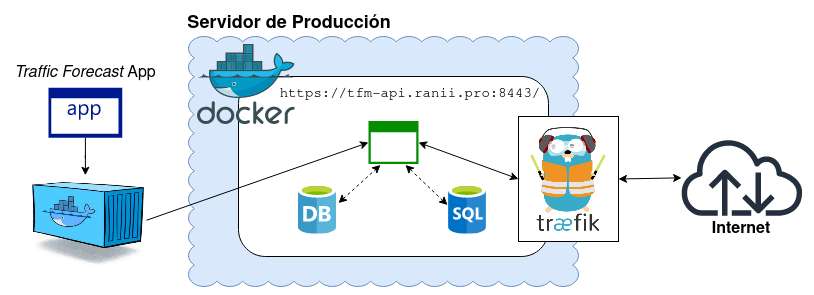
\includegraphics[width=0.95\textwidth]{diag/produccion_tfm.png}
			\end{center}
		\end{figure}
	\end{frame}
	
	% ---------------------
	
	\section{Implementación del sistema}
	
	\begin{frame}{Descripción API REST (I)}
		\begin{columns}
			\begin{column}{0.5\textwidth}
				content...
			\end{column}
		
			\begin{column}{0.5\textwidth}
				\begin{alertblock}{Agentes}
					Se identifican los diferentes ``agentes'' presentes en el sistema:
					
					\begin{itemize}
						\item \textbf{Redes} (\texttt{networks}), corresponde con una red que contiene interfaces a monitorizar.
						
						\item \textbf{Interfaces} (\texttt{interfaces}), corresponde con las interfaces de red que queremos monitorizar.
						
						\item \textbf{Muestras de monitorización} (\texttt{samples}). Valor de tráfico asociado a una interfaz en un intervalo determinado.
					\end{itemize}
				\end{alertblock}
			\end{column}
		\end{columns}
	\end{frame}
	
	% ---------------------
	
	\begin{frame}{Descripción API REST (II)}
		
		\textbf{Esquema de la aplicación implementada}
		
		\begin{figure}[h!]
			\begin{center}
				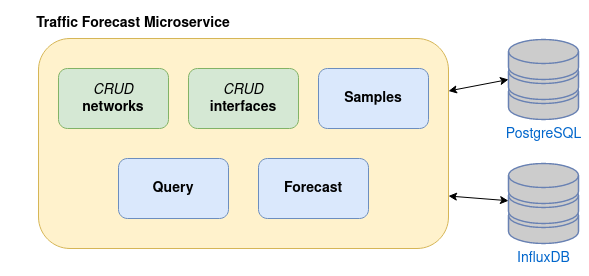
\includegraphics[width=0.75\textwidth]{diag/traffic_forecast_schema.png}
			\end{center}
		\end{figure}
	\end{frame}
	
	% ---------------------
	
	\begin{frame}{Implementación (I)}
		content...
	\end{frame}

	\begin{frame}{Implementación (II)}
		content...
	\end{frame}
	
	% ---------------------
	
	\begin{frame}{OpenAPI. Swagger}
		content...
	\end{frame}
	
	% ---------------------
	
	\begin{frame}{Modelos de datos. \texttt{SQL}}
		
		\begin{itemize}
			\item Definimos los datos y su \textbf{representación dentro} de nuestra \textbf{aplicación}.
			
			\item \textbf{En función} del \textbf{tipo de dato}, almacenaremos en \textbf{base de datos tipo relacional} (\texttt{SQL}) o \textbf{base de datos tipo serie temporal} (\texttt{InfluxDB}).
		\end{itemize}

		\vspace{11px}

		\textbf{Tablas utilizadas en la base de datos SQL}

		\begin{columns}
			\begin{column}{0.5\textwidth}
				\begin{table}[h!]
					\centering
					\begin{tabular}{|l|}
						\hline
						\multicolumn{1}{|c|}{\textit{\textbf{Networks}}} \\ \hline
						\texttt{id\_network}: Int, Public Key, Unique                 \\ \hline
						\texttt{name}: String                                     \\ \hline
						\texttt{description}: String                              \\ \hline
						\texttt{ip\_red}: String                                  \\ \hline
						\texttt{influx\_net}: String                              \\ \hline
					\end{tabular}
					%\caption{Modelo de datos para las redes a monitorizar. Equivale con la tabla \textit{networks}.}
					%\label{tab: modelo sql networks}
				\end{table}
			\end{column}
		
			\begin{column}{0.5\textwidth}
				\begin{table}[h!]
					\centering
					\begin{tabular}{|l|}
						\hline
						\multicolumn{1}{|c|}{\textit{\textbf{Interfaces}}} \\ \hline
						\texttt{id\_interface}: Int, Public Key, Unique             \\ \hline
						\texttt{name}: String                                       \\ \hline
						\texttt{description}: String                                \\ \hline
						\texttt{influx\_if\_rx}: String                             \\ \hline
						\texttt{influx\_if\_tx}: String                             \\ \hline
						\texttt{network}: Int, Foreign Key                          \\ \hline
					\end{tabular}
					%\caption{Modelo de datos para las interfaces a monitorizar. Equivale con la tabla \textit{interfaces}.}
					%\label{tab: modelo sql interfaces}
				\end{table}
			\end{column}
		\end{columns}
	\end{frame}

	\begin{frame}{Modelos de datos. \texttt{InfluxDB}}
		\begin{itemize}
			\item En \texttt{InfluxDB} almacenamos las muestras de tráfico en red.
		\end{itemize}
	
		\vspace{11px}
	
		\textbf{Configuración InfluxDB para el sistema}
	
		\begin{table}[]
			\centering
			\begin{tabular}{|c|c|}
				\hline
				\textbf{InfluxDB}    & \textbf{Descripción}                                                                                                                            \\ \hline
				\texttt{measurement} & \begin{tabular}[c]{@{}c@{}}Red a monitorizar, \\ valor almacenado en \texttt{Networks::influx\_net}\end{tabular}                                         \\ \hline
				\texttt{fields}      & Nombre del valor a monitorizar (\textit{link\_count})                                                                                                    \\ \hline
				\texttt{tags}        & \begin{tabular}[c]{@{}c@{}}Solo disponemos un tag, llamado interface, \\ contiene la información del identificador de una interfaz\end{tabular} \\ \hline
				\texttt{points}      & Corresponde con el valor numérico del campo field.                                                                                              \\ \hline
			\end{tabular}
			%\caption{}
			%\label{tab:my-table}
		\end{table}
	
	\end{frame}
	
	% ---------------------
	
	\begin{frame}{Predicción de tráfico de red}
		content...
	\end{frame}
	
	% ---------------------
	
	\begin{frame}{Resumen rutas HTTP (I)}
		\begin{columns}
			\begin{column}{0.5\textwidth}
				\begin{block}{\textbf{CRUD}: \texttt{networks} (\texttt{/networks})}
					\begin{itemize}
						\item \textbf{Información} de \textbf{todas} las redes: \\ \textit{GET} - \texttt{/networks}
						
						\item \textbf{Crear} una red: \\ \textit{POST} - \texttt{/networks}
						
						\item \textbf{Información} de \textbf{una} red: \\ \textit{GET} - \texttt{/networks/<net\_id>}
						
						\item \textbf{Eliminar} una red: \\ \textit{DELETE} - \texttt{/networks/<net\_id>}
						
						\item \textbf{Actualizar} una red: \\ \textit{PATCH} - \texttt{/networks/<net\_id>}
					\end{itemize}
				\end{block}
			\end{column}
		
			\begin{column}{0.5\textwidth}
				\begin{block}{\textbf{CRUD}: \texttt{interfaces} (\texttt{/networks/<id1>/interfaces})}
					\begin{itemize}
						\item \textbf{Información} de \textbf{todas} las interfaces: \\ \textit{GET} - \texttt{\small /networks/id/interfaces}
						
						\item \textbf{Crear} una interfaz: \\ \textit{POST} - \texttt{\small /networks/id/interfaces}
						
						\item \textbf{Información} de \textbf{una} interfaz: \\ \textit{GET} - \texttt{/../interfaces/<id2>}
						
						\item \textbf{Eliminar} una interfaz: \\ \textit{DELETE} - \texttt{/../interfaces/<id2>}
						
						\item \textbf{Actualizar} una interfaz: \\ \textit{PATCH} - \texttt{/../interfaces/<id2>}
					\end{itemize}
				\end{block}
			\end{column}
		
		\end{columns}
	\end{frame}

	\begin{frame}{Resumen rutas HTTP (II)}
		\begin{columns}
			\begin{column}{0.5\textwidth}
				\begin{block}{\texttt{Samples}}
					\begin{itemize}
						\item \textbf{Importar} datos de topología con \textbf{más de una interfaz}: \\ \textit{\small POST} - \texttt{\small /samples/id/import\_topology}
						
						\item \textbf{Importar} datos de \textbf{una interfaz}: \\ \textit{POST} - \texttt{\small /samples/id/import\_interface/id}
					\end{itemize}
				\end{block}
			\end{column}
		
			\begin{column}{0.5\textwidth}
				\begin{block}{\texttt{Query Samples}}
					\begin{itemize}
						\item \textbf{Consultar} \textbf{datos} de monitorización \textbf{almacenados}: \\ \textit{GET} - \texttt{\small /query/}
					\end{itemize}
				\end{block}
			
				\begin{block}{\texttt{Forecast}}
					\begin{itemize}
						\item \textbf{Ejecutar} \textbf{predicción} de tráfico en red: \\ \textit{POST} - \texttt{\small /forecast/}
					\end{itemize}
				\end{block}
			\end{column}
		\end{columns}
	\end{frame}
	
	% ---------------------
	
	\section{Validación del sistema}
	
	\begin{frame}{Validación del sistema (I)}
		content...
		
		\begin{exampleblock}{Demo}
			content...
		\end{exampleblock}
	\end{frame}

	\begin{frame}{Validación del sistema (II)}
		content...
	\end{frame}
	
	% ---------------------
	
	\section{Conclusiones}
	
	\begin{frame}{Conclusiones}
		\begin{itemize}
			\item Alcanzados todos los objetivos propuestos.
			
			\item Se ha desarrollado una \textbf{microservicio completo}, permitiendo ser implementado por otras aplicaciones.
			
			\item El sistema es \textbf{capaz} de \textbf{almacenar} muestras de monitorización, además de poder \textbf{generar predicciones} de tráfico en red en la escala temporal que el usuario solicite.
		\end{itemize}
	
		\begin{exampleblock}{Propuestas futuras}
			\begin{itemize}
				\item Permitir la \textbf{importación} de \textbf{datos de monitorización} de \textbf{herramientas especificas} de planificación de red.
				
				\item Añadir \textbf{funcionalidad de SSE} (Server Side Event) para \textbf{tareas} que requieran un \textbf{largo tiempo de ejecución}.
				
				\item Extender la funcionalidad de las \textbf{predicciones}, permitiendo hacer selección \textbf{más selectiva}, o añadir \textbf{filtrados extra}.
			\end{itemize}
		\end{exampleblock}
	\end{frame}
	
	% ---------------------
	
	\section{Bibliografía}
	
	\begin{frame}{Bibliografía}
		\begin{itemize}
		    \item La contenida en la memoria del proyecto: páginas 53 - 54
		\end{itemize}
	\end{frame}
	
	\begin{frame}
	    \begin{center}
	        \vspace{30px}
	        \Large \textbf{Muchas gracias por su atención} \\
	        \vspace{30px}
	        \large ¿Preguntas? \\
	        \vspace{60px}
	        
	        Enlace a la aplicación: \\
	        \href{https://tfm-api.ranii.pro:8443/docs}{\texttt{https://tfm-api.ranii.pro:8443/}}
	    \end{center}
	\end{frame}
	
\end{document}